\documentclass[answers]{exam}
\usepackage{marvosym}

%...TikZ & PGF
\usepackage{pgfplots}
\pgfplotsset{compat=1.11}
\tikzset{>=latex}
\usetikzlibrary{calc,math}
\usepackage{tikzsymbols}
\usepgfplotslibrary{fillbetween}
\usetikzlibrary{decorations.markings} 
\usetikzlibrary{arrows.meta} %...APP2 for arrows as objects and images
\usetikzlibrary{backgrounds} %...For shading portions of graphs
\usetikzlibrary{patterns} %...Unit 5 Problems
\usetikzlibrary{shapes.geometric} %...For drawing cylinders in Unit 2
\tikzset{
    mark position/.style args={#1(#2)}{
        postaction={
            decorate,
            decoration={
                markings,
                mark=at position #1 with \coordinate (#2);
            }
        }
    }
} %...See https://tex.stackexchange.com/questions/43960/define-node-at-relative-coordinates-of-draw-plot

\tikzset{
    declare function = {trajectoryequation10(\x,\vi,\thetai)= tan(\thetai)*\x - 10*\x^2/(2*(\vi*cos(\thetai))^2);},
    declare function = {trajectoryequation(\x,\vi,\thetai)= tan(\thetai)*\x - 9.8*\x^2/(2*(\vi*cos(\thetai))^2);},
    declare function = {patheq(\x,\yi,\vi,\thetai)= \yi + tan(\thetai)*\x - 9.8*\x^2/(2*(\vi*cos(\thetai))^2);},
    declare function = {patheqten(\x,\yi,\vi,\thetai)= \yi + tan(\thetai)*\x - 10*\x^2/(2*(\vi*cos(\thetai))^2);} %like patheq but with gravity = 10
}

%...siunitx
\usepackage{siunitx}
\DeclareSIUnit{\nothing}{\relax}
\def\mymu{\SI{}{\micro\nothing} }
\DeclareSIUnit\mmHg{mmHg}
\DeclareSIUnit{\mile}{mi}
%...NOTE: "The product symbol between the number and unit is set using the quantity-product option."

%...Other
\usepackage{amsthm}
\usepackage{amsmath}
\usepackage{amssymb}
\usepackage{cancel}
\usepackage{subcaption}
\usepackage{dashrule}
\usepackage{enumitem}
\usepackage{fontawesome}
\usepackage{multicol}
\usepackage{glossaries}
%\numberwithin{equation}{section}
\numberwithin{figure}{section}
\usepackage{float}
\usepackage{twemojis} %...twitter emojis
\usepackage{utfsym}
\newcommand{\R}{\mathbb{R}} %...real number symbol
\usepackage{graphicx}
\graphicspath{ {../Figures/} }
\usepackage{hyperref}
\hypersetup{colorlinks=true,
    linkcolor=blue,
    filecolor=magenta,
    urlcolor=cyan,}
\urlstyle{same}
\newcommand{\hdashline}{{\hdashrule{\textwidth}{0.5pt}{0.8mm}}}
\newcommand{\hgraydashline}{{\color{lightgray} \hdashrule{0.99\textwidth}{1pt}{0.8mm}}}

%...Miscellaneous user-defined symbols
\newcommand{\fnet}{F_{\text{net}}} %...For net force
\newcommand{\bvec}[1]{\vec{\mathbf{#1}}} %...bold vector
\newcommand{\bhat}[1]{\,\hat{\mathbf{#1}}} %...bold hat vector
\newcommand{\que}{\mathord{?}}  %...Question mark symbol in equation env
%...Define thick horizontal rule for examples:
\newcommand{\hhrule}{\hrule\hrule}
\let\oldtexttt\texttt% Store \texttt
\renewcommand{\texttt}[2][black]{\textcolor{#1}{\ttfamily #2}}% 

%...For use in the exam document class
\newif\ifprintmetasolutions


%...Decreases space above and below align and gather enironment
\makeatletter
\g@addto@macro\normalsize{%
  \setlength\abovedisplayskip{-3pt}
  \setlength\belowdisplayskip{6pt} 
}
\makeatother





\usepackage[margin=1in]{geometry}
\usepackage[figurewithin=none]{caption}
\usepackage{exam-randomizechoices}

\CorrectChoiceEmphasis{\color{red}\bfseries}
\renewcommand{\solutiontitle}{\noindent\textbf{\textcolor{red}{Solution:}}\enspace}

\usepackage{OutilsGeomTikz}
\usepackage{utfsym} %...Symbols in Unit 7 Problems
\usepackage{tabu} %...Symbols in Unit 7 Problems

%...For use in Unit 2            %    
\setlength{\columnsep}{2cm}      %
\setlength{\columnseprule}{1pt}  %
\usepackage[none]{hyphenat}      %
%%%%%%%%%%%%%%%%%%%%%%%%%%%%%%%%%

%...For use in Unit 11 on Waves:
\pgfdeclarehorizontalshading{visiblelight}{50bp}{  %
color(0.00000000000000bp)=(red);                   %
color(8.33333333333333bp)=(orange);                %
color(16.66666666666670bp)=(yellow);               %
color(25.00000000000000bp)=(green);                %
color(33.33333333333330bp)=(cyan);                 %
color(41.66666666666670bp)=(blue);                 %
color(50.00000000000000bp)=(violet)                %
}                                                  %

\newcommand{\checkbox}[1]{%
  \ifnum#1=1
    \makebox[0pt][l]{\raisebox{0.15ex}{\hspace{0.1em}\Large$\checkmark$}}%
  \fi
  $\square$%
}
%%%%%%%%%%%%%%%%%%%%%%%%%%%%%%%%%%%%%%%%%%%%%%%%%%%%

%...If using circuitikz package:
% \ctikzset{bipoles/battery1/height=0.5}
% \ctikzset{bipoles/battery1/width=0.25}
% \ctikzset{bipoles/resistor/height=0.15}
% \ctikzset{bipoles/resistor/width=0.4}
\usepackage{mdframed}

\setrandomizerseed{2}
\bracketedpoints
\addpoints

\newif\ifversionKlevel

\versionKleveltrue

\header{Physics L\\Test on Unit 5: Force Analysis}{}{Name:\enspace\makebox[5cm]{\hrulefill}}

\ifversionKlevel
    \header{Physics K\\Test on Unit 5: Force Analysis}{}{Name:\enspace\makebox[5cm]{\hrulefill}}
\fi

\begin{document}
\begin{questions}
\question 
A physics textbook that weighs \SI{25.0}{N} rests on a table. What is the normal force the table exerts on the textbook?

\begin{randomizeoneparchoices}[norandomize]
    \choice \SI{0}{N}
    \correctchoice \SI{25.0}{N}
    \choice \SI{9.80}{N}
    \choice \SI{12.0}{N}
\end{randomizeoneparchoices}

\question 
What is the weight of an 12 kilogram object on the surface of Earth?

\begin{randomizeoneparchoices}[norandomize]
    \choice \SI{6}{N}
    \choice \SI{10}{N}
    \correctchoice \SI{120}{N}
    \choice \SI{480}{N}
\end{randomizeoneparchoices}

\question
Which equation correctly describes the net force acting in the horizontal direction? 

\begin{center}
    \begin{tikzpicture}
        \fill (0,0) circle (3pt);
        \draw [<->] (-1,0) node[left] {$F_\mathrm{f}$} -- (+1,0) node[right] {$F_\mathrm{A}$};
        \draw [<->] (0,-1) node[below] {$F_\mathrm{g}$} -- (0,+1) node[above] {$F_\mathrm{N}$};
    \end{tikzpicture}
\end{center}

\begin{randomizechoices}[norandomize]
    \choice $F_\mathrm{net} = F_\mathrm{N} + F_\mathrm{A}$
    \choice $F_\mathrm{net} = F_\mathrm{N} + F_\mathrm{g}$
    \choice $F_\mathrm{net} = F_\mathrm{N} - F_\mathrm{g}$
    \correctchoice $F_\mathrm{net} = F_\mathrm{A} - F_\mathrm{f}$
\end{randomizechoices}

\question 
Peter Parker pulls a sled carrying MJ to the right at a constant speed. MJ then jumps off the sled while Peter is still pulling the sled. How does the magnitude of the friction force after MJ jumped off the sled compare to the friction force before?

\begin{randomizechoices}[norandomize]
    \choice Increases
    \choice Remains the same
    \correctchoice Decreases
    \choice Not enough information to determine    
\end{randomizechoices}

\question 
Three objects with the same mass are sliding across a rough surface with no applied forces acting on any of them. The velocity vs time graph shown below depicts their motion. Which object experiences the greatest friction force?

\begin{center}
    \begin{tikzpicture}
        \begin{axis}[width=8cm,
            height=6cm,
            xmin=0,xmax=25,
            ymin=-10,ymax=10,
            ylabel={Velocity (m/s)},
            xlabel={Time (s)},
            grid=both,
            axis lines=middle,
            xtick={0,5,...,25},
            ytick={-10,-5,...,10},
            y label style={at={(axis description cs:-0.15,.5)},rotate=90,anchor=south},
            x label style={at={(axis description cs:1,.5)},anchor=west},
            % minor tick num=4,
            ]
            \draw[thick] (0,10) -- (10,0) node[above=2pt,pos=0.9] {\bfseries A};
            \draw[thick] (0,10) -- (25,0) node[above=2pt,pos=0.9] {\bfseries B};
            \draw[thick] (0,10) -- (25,5) node[above=2pt,pos=0.9] {\bfseries C};
        \end{axis}
    \end{tikzpicture}
\end{center}

\begin{randomizechoices}[norandomize]
    \correctchoice Object A
    \choice Object B
    \choice Object C
    \choice Cannot determine from graph
\end{randomizechoices}


\question
When an object is transported from Earth to the Moon

\begin{randomizechoices}[norandomize]
    \choice its weight and its mass will not change
    \choice its weight and its mass will change
    \correctchoice its weight changes and its mass does not
    \choice its weight stays the same and its mass changes    
\end{randomizechoices}


\question 
This graph shows weight versus mass for a group of objects on planet X.

\begin{center}
    \begin{tikzpicture}
        \begin{axis}[width=6cm,
            height=6cm,
            xmin=0,xmax=16,
            ymin=0,ymax=26,
            xlabel={Mass (kg)},
            ylabel={Weight (N)},
            xtick={0,2,...,16},
            ytick={0,4,...,26},
            minor tick num=1,
            grid=both,
            axis lines=left,
        ]
            % \addplot[color=black,thick,mark=*]
            %     coordinates{(2,4)(8,16)(12,24)};
            % \draw[thick] (0,0) -- (2,4);
            \addplot[very thick,domain=0:16] {0.5*x};
        \end{axis}
    \end{tikzpicture}
\end{center}

What is the acceleration due to gravity on planet X?

\begin{randomizechoices}[norandomize]
    \correctchoice \SI{0.5}{m/s^2}
    \choice \SI{10}{m/s^2}
    \choice \SI{2}{m/s^2}
    \choice \SI{6}{m/s^2}
\end{randomizechoices}

\question
A free-body diagram of a ball falling with air resistance would show

\begin{center}
    \begin{tikzpicture}
        \node at (0,0) {\twemoji[height=1cm]{tennis}};
        \draw[black!80] (-0.6,0.2) -- ++(0,1)
                        (+0.6,0.2) -- ++(0,1)
                        (+0.75,0.4) -- ++(0,0.5)
                        (-0.75,0.4) -- ++(0,0.5);
    \end{tikzpicture}
\end{center}

\begin{randomizechoices}[norandomize]
    \choice an upward arrow to represent the force of gravity and a downward arrow to represent the force of air resistance.
    \choice only a downward arrow to represent the force of gravity.
    \correctchoice a downward arrow to represent the force of gravity and an upward arrow to represent the force of air resistance.
    \choice a downward arrow to represent the force of air resistance.
\end{randomizechoices}


\clearpage
\question
Which diagram best represents the gravitational forces, $F_g$, between a satellite, S, and Earth?

\begin{center}
    \begin{tikzpicture}
        \draw[->,white] (0,0) -- (0,-0.6-0.6) node[right] {$F_g$}; %...for scaling; don't erase
        \draw[->] (0,0) -- (0,+0.6+0.6) node[right] {$F_g$};
        \draw[fill=white] (0,0) circle (6mm) node {Earth};
        \begin{scope}[yshift=2.8cm]
            \draw[->,white] (0,0) -- (0,0.3+0.6) node[right] {$F_g$}; %...for scaling; don't erase
            \draw[->] (0,0) -- (0,-0.3-0.6) node[right] {$F_g$};
            \draw[fill=white] (0,0) circle (3mm) node {S};
            \node at (0,1.5) {\bfseries Diagram A};
        \end{scope}
    \end{tikzpicture}
    \hspace{2em}
    \begin{tikzpicture}
        \draw[->] (0,0) -- (0,-0.6-0.6) node[right] {$F_g$};
        \draw[fill=white] (0,0) circle (6mm) node {Earth};
        \begin{scope}[yshift=2.8cm]
            \draw[->,white] (0,0) -- (0,0.3+0.6) node[right] {$F_g$}; %...for scaling; don't erase
            \draw[->] (0,0) -- (0,-0.3-0.6) node[right] {$F_g$};
            \draw[fill=white] (0,0) circle (3mm) node {S};
            \node at (0,1.5) {\bfseries Diagram B};
        \end{scope}
    \end{tikzpicture}
    \hspace{2em}
    \begin{tikzpicture}
        \draw[->] (0,0) -- (0,-0.6-0.6) node[right] {$F_g$};
        \draw[fill=white] (0,0) circle (6mm) node {Earth};
        \begin{scope}[yshift=2.8cm]
            \draw[->] (0,0) -- (0,0.3+0.6) node[right] {$F_g$};
            \draw[fill=white] (0,0) circle (3mm) node {S};
            \node at (0,1.5) {\bfseries Diagram C};
        \end{scope}
    \end{tikzpicture}
    \hspace{2em}
    \begin{tikzpicture}
        \draw[->,white] (0,0) -- (0,-0.6-0.6) node[right] {$F_g$}; %...for scaling; don't erase
        \draw[->] (0,0) -- (0,+0.6+0.6) node[right] {$F_g$};
        \draw[fill=white] (0,0) circle (6mm) node {Earth};
        \begin{scope}[yshift=2.8cm]
            \draw[->] (0,0) -- (0,0.3+0.6) node[right] {$F_g$};
            \draw[fill=white] (0,0) circle (3mm) node {S};
            \node at (0,1.5) {\bfseries Diagram D};
        \end{scope}
    \end{tikzpicture}
\end{center}

{\color{white} \tiny
\begin{randomizeoneparchoices}[norandomize]
    \correctchoice Diagram A \hspace{1cm}
    \choice Diagram B \hspace{1cm}
    \choice Diagram C \hspace{1cm}
    \choice Diagram D \hspace{1cm}
\end{randomizeoneparchoices}
}

\question
According to the Newton’s Law of Universal Gravitation, when the distance between any two objects decreases, the force of gravity between the two objects

\begin{randomizechoices}[norandomize]
    \choice not enough information
    \correctchoice increases
    \choice decreases
    \choice stays the same    
\end{randomizechoices}


\question %...NOTE: The original problem read, ``As a meteor moves from a distance of \SI{6000}{km} to a distance of \SI{3000} km from the center of Earth, the magnitude of the gravitational force between the meteor and Earth becomes...'' This problem is physically unreasonable, since Earth's radius is 6378 km, which immplies the meteor would be traveling inside of Earth. So, the numbers below have been changed to conform to reality.

As a meteor moves from a distance of \SI[group-separator={,}]{20000}{km} to a distance of \SI[group-separator={,}]{10000}{km} from the center of Earth, the magnitude of the gravitational force between the meteor and Earth becomes

\begin{randomizeoneparchoices}[norandomize]
    \correctchoice 4 times as great
    \choice 64 times as great
    \choice 1/8 as great
    \choice 8 times as great
\end{randomizeoneparchoices}

\question
Earth’s mass is approximately 81 times the mass of the moon.  If the earth exerts a gravitational force of magnitude $F$ on the Moon, the magnitude of the gravitational force of the moon on the earth is

\begin{randomizechoices}[norandomize]
    \correctchoice the same as $F$
    \choice greater than $F$
    \choice less than $F$
    \choice not enough information to tell
\end{randomizechoices}

\bigskip
\hrule\hrule


\begin{EnvUplevel}
    \textbf{Questions \ref{Q24}--\ref{Q25}.} Use this picture and scenario below for questions \ref{Q24} and \ref{Q25}. Troy Bolton is helping his dad clean out the garage. He is pulling a box of old sports equipment with a mass of \SI{70}{kg} across the smooth floor with a force of \SI{400}{N} at an angle above the horizontal, as shown below. The horizontal component of the tension force is \SI{346}{N}.
\end{EnvUplevel}

\begin{center}
    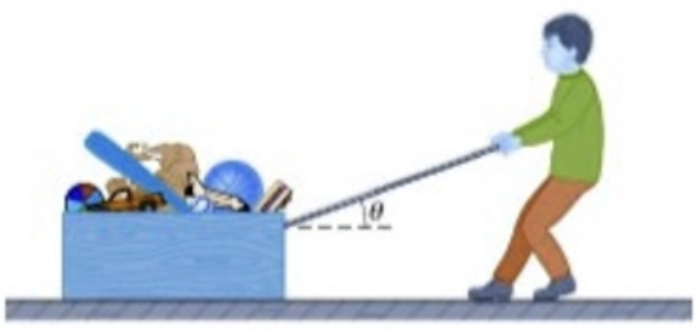
\includegraphics[width=5cm]{physics/figures/figure-unit-4-bolton.png}
\end{center}

\question \label{Q24}
What is the magnitude of the vertical component of the tension force?

\begin{randomizeoneparchoices}[norandomize]
    \choice \SI{700}{N}
    \correctchoice \SI{200}{N}
    \choice \SI{300}{N}
    \choice \SI{500}{N}
\end{randomizeoneparchoices}

\question \label{Q25}
What is the magnitude of the normal force acting on the box?

\begin{randomizeoneparchoices}[norandomize]
    \choice \SI{686}{N}
    \choice \SI{632}{N}
    \choice \SI{432}{N}
    \correctchoice \SI{500}{N}
\end{randomizeoneparchoices}
\bigskip
\hrule\hrule

\question
The diagram shows two spheres, A and B, having masses of 100 and 400 kilograms, placed 1.5 meters apart.

\begin{center}
    \begin{tikzpicture}
        \draw[fill=black!10] (0,0) circle (1) node {\SI{100}{kg}} node[above=1cm] {\textbf{A}};
        \draw[fill=black!10] (5,0) circle (1) node {\SI{400}{kg}} node[above=1cm] {\textbf{B}};
        \draw[|<->|,dashed] (0,-1.15) -- ++ (5,0) node[below,pos=0.5] {\SI{1.5}{m}};
    \end{tikzpicture}
\end{center}

What is the magnitude of the gravitational force exerted by ball A on ball B?

\begin{randomizeoneparchoices}
    \correctchoice \SI{1.2e-6}{N}
    \choice \SI{2.0e-6}{N}
    \choice \SI{1.8e4}{N}
    \choice \SI{2.7e4}{N}
\end{randomizeoneparchoices}

\ifversionKlevel
\question
In the figure below, static friction prevents a box from sliding.

\begin{center}
\begin{tikzpicture}[x=7mm,y=7mm,rotate=-37]
    \draw (0,0) -- (5,0);
    \draw[fill=black!10] (2,0) rectangle ++(1,1);
    \end{tikzpicture}
\end{center}

Which of the following is a correct free body diagram for this scenario?

\begin{center}
\begin{tikzpicture}[x=1.5cm,y=1.5cm]
    \begin{scope}[rotate=-37]
        \draw[thick,->] (0,0) -- (0,{cos(37)}) node[above] {$F_\mathrm{N}$};
        \draw[thick,->] (0,0) -- ({-sin(37)},0) node[left] {$F_f$};
    \end{scope}
    \draw[thick,->] (0,0) -- (0,-1) node[below] {$F_g$};
    \fill[black] (0,0) circle (3pt);
    \node[below=3pt] at (current bounding box.south) {Diagram A};
\end{tikzpicture}
\hspace{1cm}
\begin{tikzpicture}[x=1.5cm,y=1.5cm]
    \begin{scope}[rotate=0]
        \draw[thick,->] (0,0) -- (0,{cos(37)}) node[above] {$F_\mathrm{N}$};
        \draw[thick,->] (0,0) -- ({-sin(37)},0) node[left] {$F_f$};
    \end{scope}
    \draw[thick,->] (0,0) -- (0,-1) node[below] {$F_g$};
    \fill[black] (0,0) circle (3pt);
    \node[below=3pt] at (current bounding box.south) {Diagram B};
\end{tikzpicture}
\hspace{1cm}
\begin{tikzpicture}[x=1.5cm,y=1.5cm]
    \begin{scope}[rotate=37]
        \draw[thick,->] (0,0) -- (0,{cos(37)}) node[above] {$F_\mathrm{N}$};
        \draw[thick,->] (0,0) -- ({-sin(37)},0) node[left] {$F_f$};
    \end{scope}
    \draw[thick,->] (0,0) -- (0,-1) node[below] {$F_g$};
    \fill[black] (0,0) circle (3pt);
    \node[below=3pt] at (current bounding box.south) {Diagram C};
\end{tikzpicture}
\hspace{1cm}
\begin{tikzpicture}[x=1.5cm,y=1.5cm]
    \begin{scope}[rotate=-37]
        \draw[thick,->] (0,0) -- ({-sin(37)},0) node[left] {$F_f$};
    \end{scope}
    \draw[thick,->,white] (0,0) -- (0,-1) node[below] {$F_g$};
    \fill[black] (0,0) circle (3pt);
    \node[below=3pt] at (current bounding box.south) {Diagram D};
\end{tikzpicture}
\end{center}

{\color{white} \tiny
\begin{randomizeoneparchoices}[norandomize]
    \correctchoice A
    \choice B
    \choice C
    \choice D
\end{randomizeoneparchoices}
}


\question
The object is pulled at constant velocity by a force at an angle to the surface with friction.

\begin{center}
\begin{tikzpicture}[x=7mm,y=7mm]
    \draw (-1.5,0) -- ++(4,0);
    \draw[fill=black!10] (0,0) rectangle ++(1,1);
    \draw[thick,->] (1,1) -- ++({1.4*cos(45)},{1.4*sin(45)}) node[right] {$F$};
    \draw[dashed] (1,1) -- ++({1.4*cos(45)},0);
    \node[xshift=4.4mm,yshift=2mm] at (1,1) {\small $\theta$};
    \ifprintanswers
    \color{red}
    \else
    \color{white}
    \fi
    \begin{scope}[xshift=4cm,x=2cm,y=1.5cm,yshift=0.75cm]
        \draw[thick,->,xshift=1.5pt] (0,0) -- (0,{1-0.8*sin(45)}) node[right] {$F_\mathrm{N}$};
        \draw[thick,->] (0,0) -- (0,-1) node[below] {$F_g$};
        \draw[thick,->,xshift=-1.5pt] (0,0) -- ++(0,{0.8*sin(45)}) node[left] {$F_y$};
        \draw[thick,->] (0,0) -- ({0.8*cos(45)},0) node[right] {$F_x$};
        \draw[thick,->] (0,0) -- ({-0.8*cos(45)},0) node[left] {$F_f$};
        \fill[black] (0,0) circle (4pt);
    \end{scope}
\end{tikzpicture}
\end{center}

Which of the following represents the net force equation in the vertical direction?

\begin{randomizechoices}
    \correctchoice $F_{\mathrm{net},y} = F_\mathrm{N} + F_y - F_g = 0$
    \choice $F_{\mathrm{net},y} = F_\mathrm{N} - F_g = 0$
    \choice $F_{\mathrm{net},y} = F_y - F_g = 0$
    \choice $F_{\mathrm{net},y} = F_\mathrm{N} - F_y - F_g = 0$
\end{randomizechoices}
\fi

\clearpage

\begingradingrange{myrange} 
\question[6]
Mia is pulling up a \SI{25}{kg} bucket of water with an acceleration of \SI{3}{m/s^2} to quench her thirst. 

\begin{center}
    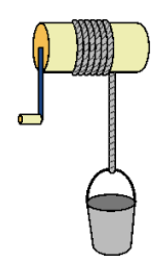
\includegraphics[width=2cm]{physics/figures/figure-unit-4-bucket.png}
\end{center}

\begin{parts}
\part Using the dot below, draw a free body diagram with all the forces acting on the bucket.

\begin{center}
\begin{tikzpicture}
    \ifprintanswers
        \color{red}
    \else
        \color{white}
    \fi
    \draw[thick,->] (0,0) -- (0,1.2) node[above] {$F_\mathrm{T}$};
    \draw[thick,->] (0,0) -- (0,-0.8) node[below] {$F_g$};
    \fill[black] (0,0) circle (3pt);
\end{tikzpicture}
\end{center}

% \begin{solutionorbox}[4cm]

% \end{solutionorbox}

\part Write the $F_\mathrm{net}$ equation for the bucket.
\vspace{-1ex}

{\Large
\begin{equation*}
    F_{\mathrm{net},y} = 
    {\ifprintanswers \color{red} F_\mathrm{T} - F_g = m a_y \fi}
\end{equation*}
}
\vspace{1ex}

\part Solve for the tension in the cable as the bucket is being pulled up.

\begin{solutionorbox}[7cm]
If $F_\mathrm{T} - F_g = ma_y$, then
\vspace{-1em}

\begin{align*}
    F_\mathrm{T} &= ma_y + F_g \\[1ex]
    &= ma_y + mg \\[1ex]
    &= (\SI{25}{kg})(\SI{3}{m/s^2}) + (\SI{25}{kg})(\SI{10}{N/kg}) \\[1ex]
    &= \boxed{\SI{325}{N}}
\end{align*}
\end{solutionorbox}
\end{parts}

\vspace*{\fill}

\ifprintanswers
\else
\begin{mdframed}[backgroundcolor=black!10]
    \centering
    \textbf{\small TEACHER USE ONLY}\\[1em]
    \partialgradetable{myrange}[h][questions]
\end{mdframed}
\fi



\clearpage

\question[2]
The figure below shows the same rocket at two different positions, P and Q, relative to a planet. When the rocket is located at Point P, the gravitational force on the rocket by the planet is \SI{72}{N}. 

\ifversionKlevel
%%%% K-LEVEL FIGURE %%%%%
    \begin{center}
    \begin{tikzpicture}
        \draw[step=1cm,gray] (0,0) grid (8,6);
        \node[opacity=0.8] at (6,2) {\twemoji[width=2cm]{globe showing Americas}};
        \draw[->, very thick] (0,5) node[above right=1pt] {P} -- ++(6*0.4,-3*0.4) node[below] {\SI{72}{N}}; 
        \draw  (0,5) node[rotate=100] {\twemoji[width=4mm]{rocket}};
        \fill  (6,2) ++(-3,0) circle (3pt) node[below left] {Q};
    \end{tikzpicture}
    \end{center}
\else

%%%% L-LEVEL FIGURE %%%%%
\begin{center}
\begin{tikzpicture}
    \draw[step=1cm,gray] (0,0) grid (8,4);
    \node[opacity=0.8] at (7,2) {\twemoji[width=2cm]{globe showing Americas}};
    \draw[->,very thick] (4,2) -- ++(1.5,0) node[above] {\SI{72}{N}};
    \draw  (4,2)  node[rotate=135] {\twemoji[width=4mm]{rocket}} node[below left=1pt] {P};
    \fill  (1,2) circle (3pt) node[below left] {Q};
\end{tikzpicture}
\end{center}
\fi


(a) Use a checkmark below to indicate whether the magnitude of the gravitational force increases, decreases, or stays the same when the rocket moves from Point P to Point Q. 

\begin{center}
    \large
\ifversionKlevel
    \fillin[{\huge \checkmark}][1cm]\ \textbf{increases} \hspace{2em}
    \fillin[][1cm]\ \textbf{decreases} \hspace{2em}
    \fillin[][1cm]\ \textbf{stays the same}
\else
    \fillin[][1cm]\ \textbf{increases} \hspace{2em}
    \fillin[{\huge \checkmark}][1cm]\ \textbf{decreases} \hspace{2em}
    \fillin[][1cm]\ \textbf{stays the same}
\fi
\end{center}


(b) Find the magnitude of the gravitational force, in newtons (N), on the rocket when it is at Point Q.

\ifversionKlevel
    \begin{solutionorbox}[7cm]
    The distance between Q and the center of Earth is 3 grid units. The distance between P and the center of the Earth is $\sqrt{6^2 + 3^2}$ units. So, the distance between P and Q decreases by a factor of 
    
    \begin{equation*}
        \frac{r}{r_0} = \frac{3}{\sqrt{6^2 + 3^2}}
    \end{equation*}
    
    By Newton's universal law of gravitation,
    
    \begin{equation*}
        F_g = \frac{Gm_1 m_2}{r^2}
    \end{equation*}
    
    force is inversely proportional to distance squared. So, at point Q the original force is change by a factor of 
    
    \begin{equation*}
        F_\mathrm{Q} \propto \frac{1}{\left(\displaystyle \frac{r}{r_0}\right)^2} = \frac{1}{\left(\displaystyle \frac{3}{\sqrt{6^2 + 3^2}}\right)^2}
    \end{equation*}
    
    Therefore, the the force a Q is
    
    \begin{equation*}
        F_\mathrm{Q} = F_\mathrm{P} \times \frac{1}{\left(\displaystyle \frac{3}{\sqrt{6^2 + 3^2}}\right)^2} = \SI{72}{N} \times \frac{1}{\left(\displaystyle \frac{3}{\sqrt{6^2 + 3^2}}\right)^2} = \boxed{\SI{360}{N}}
    \end{equation*}
    \end{solutionorbox}
\else
    \begin{solutionorbox}[10cm]
    The distance between the P and the center of Earth is 3 grid units. The distance between Q and the center of Earth is 6 units. So, the distance between P and Q increases by a factor of 
    
    \begin{equation*}
        \frac{r}{r_0} = \frac{6}{3} = \frac{2}{1}
    \end{equation*}
    
    By Newton's universal law of gravitation,
    
    \begin{equation*}
        F_g = \frac{Gm_1 m_2}{r^2}
    \end{equation*}
    
    force is inversely proportional to distance squared. So, at point Q the original force is change by a factor of 
    
    \begin{equation*}
        F_\mathrm{Q} \propto \frac{1}{\left(\displaystyle \frac{r}{r_0}\right)^2} = \frac{1}{\left(\displaystyle \frac{2}{1}\right)^2}
    \end{equation*}
    
    Therefore, the the force a Q is
    
    \begin{equation*}
        F_\mathrm{Q} = F_\mathrm{P} \times \frac{1}{\left(\displaystyle \frac{2}{1}\right)^2} = \SI{72}{N} \times \frac{1}{\left(\displaystyle \frac{2}{1}\right)^2} = \boxed{\SI{18}{N}}
    \end{equation*}
    \end{solutionorbox}
\fi



\ifversionKlevel

\ifprintanswers
    \clearpage
\fi

\question[2]
The object below is accelerated rightward by an applied force parallel to the rough surface. Friction is significant. Draw the free-body diagram, and write the net force equations in horizontal and vertical directions.

\begin{center}
\begin{minipage}[c][4cm][c]{0.5\textwidth}
\begin{tikzpicture}[x=7mm,y=7mm,remember picture]
    \draw (-1.5,0) -- ++(4,0);
    \draw[fill=black!10] (0,0) rectangle ++(1,1);
    \draw[thick,->] (1,0.5) -- ++(1.2,0) node[right] {$F$};
    \ifprintanswers
    \color{red}
    \else
    \color{white}
    \fi
    \begin{scope}[xshift=4.5cm,x=1cm,y=1cm]
        \draw[thick,->] (0,0) -- (0,+1) node[above] {$F_\mathrm{N}$};
        \draw[thick,->] (0,0) -- (0,-1) node[below] {$F_g$};
        \draw[thick,->] (0,0) -- (1.5,0) node[right] {$F$};
        \draw[thick,->] (0,0) -- (-0.7,0) node[left] {$F_f$};
        \fill[black] (0,0) circle (3pt);  
    \end{scope}
\end{tikzpicture}
\end{minipage}%
\hspace{2em}
\begin{minipage}[c][4cm][c]{0.35\textwidth}
    \Large
    \begin{align*}
        F_{\mathrm{net},x} &= {\ifprintanswers \color{red} F - F_f = m a_x \fi} \\[1ex]
        F_{\mathrm{net},y} &= {\ifprintanswers \color{red} F_\mathrm{N}  - F_g = 0 \fi}
    \end{align*}
\end{minipage}
\end{center}
\fi

\endgradingrange{myrange} 

\ifprintanswers
    \printkeytable
\fi






\end{questions}
\end{document}